\begin{homeworkProblem}
  Sea
    \begin{equation}
       A=\begin{pmatrix}
          0 & -20 & 14\\
          -3 & 27 & 4\\
          -4 & 11 & 2
       \end{pmatrix}
    \end{equation}
    \begin{itemize}
        \item[a)] Aplique las transformaciones de Householder, para calcular $A=QR$.
        \begin{solucion}
          Sea $A$ una matriz de tamaño $3\times 3$. Buscamos descomponerla como $A=QR$, donde $Q$ es una matriz ortogonal y $R$ una matriz triangular superior, ambas de tamaño $3\times3$.\\
    
    Como primer paso, tomemos la primera columna de $A$, que llamaremos $a_1=(0, -3, -4)^{T}$, y definamos el vector de Householder $v_1$:
    \begin{align*}
        v_1 &= a_1 + \text{sign}(a_{11}) \|a_1\| e_1\\
        &= (0, -3, -4)^{T} + \|(0, -3, -4)^{T}\| (1,0, 0)^{T} \\
        &= (0, -3, -4)^{T} + 5 (1,0, 0)^{T}\\
        &= (5,-3,-4)^{T}
    \end{align*}

    A continuación, calculemos $v^{T}v$ y el producto exterior $v v^{T}$:
    \begin{align*}
        v^{T}v &= \begin{pmatrix} 5 & -3 & -4 \end{pmatrix}
        \begin{pmatrix} 5\\ -3\\ -4\\ \end{pmatrix} = 50\\
        v v^{T} &= \begin{pmatrix} 5\\ -3\\ -4 \end{pmatrix}
        \begin{pmatrix} 5 & -3 & -4 \end{pmatrix} =
        \begin{pmatrix}
            25 & -15 & -20\\
            -15 & 9 & 12\\
            -20 & 12 & 16
        \end{pmatrix}
    \end{align*}

    Ahora calculamos la matriz de Householder correspondiente:
    \begin{align*}
        F_1 &= I - \frac{2}{v^T v} v v^{T}\\
        &= \begin{pmatrix} 1&0&0\\ 0&1&0\\ 0&0&1 \end{pmatrix} 
        - \frac{2}{50} 
        \begin{pmatrix}
            25 & -15 & -20\\
            -15 & 9 & 12\\
            -20 & 12 & 16
        \end{pmatrix}\\
        &= \begin{pmatrix}
            0 & \frac{3}{5} & \frac{4}{5}\\
            \frac{3}{5} & \frac{16}{25} & -\frac{12}{25}\\
            \frac{4}{5} & -\frac{12}{25} & \frac{9}{25}
        \end{pmatrix}
    \end{align*}

    Aplicamos $F_1$ a $A$ para introducir ceros debajo de la primera entrada:
    \begin{align*}
        F_1 A = 
        \begin{pmatrix}
            0 & \frac{3}{5} & \frac{4}{5}\\
            \frac{3}{5} & \frac{16}{25} & -\frac{12}{25}\\
            \frac{4}{5} & -\frac{12}{25} & \frac{9}{25}
        \end{pmatrix}
        \begin{pmatrix}
            0 & -20 & 14\\
            -3 & 27 & 4\\
            -4 & 11 & 2
        \end{pmatrix}
        =
        \begin{pmatrix}
            -5 & 25 & 4\\
            0 & 0 & 10\\
            0 & -25 & 10
        \end{pmatrix}
    \end{align*}

    Ahora tomamos la submatriz inferior derecha de $F_1 A$, denotada por:
    \[
    A^{(2)} =
    \begin{pmatrix}
        0 & 10\\
        -25 & 10
    \end{pmatrix}
    \]
    y repetimos el proceso anterior para $a_2=(0, -25)^{T}$. Definimos entonces $v_2$:
    \begin{align*}
        v_2 &= (0, -25)^{T} + \|(0, -25)^{T}\|(1, 0)^{T} \\
        &= (25, -25)^{T}
    \end{align*}

    Calculamos su norma y el producto exterior:
    \begin{align*}
        v_2^{T} v_2 &= \begin{pmatrix} 25 & -25 \end{pmatrix}
        \begin{pmatrix} 25\\ -25 \end{pmatrix} = 1250\\
        v_2 v_2^{T} &= \begin{pmatrix} 25\\ -25 \end{pmatrix}
        \begin{pmatrix} 25 & -25 \end{pmatrix} =
        \begin{pmatrix}
            625 & -625 \\
            -625 & 625
        \end{pmatrix}
    \end{align*}

    Entonces, la nueva matriz de Householder es:
    \begin{align*}
        F_2 &= \begin{pmatrix} 1 & 0 \\ 0 & 1 \end{pmatrix}
        - \frac{2}{1250}
        \begin{pmatrix}
            625 & -625 \\
            -625 & 625
        \end{pmatrix} \\
        &= \begin{pmatrix}
            0 & 1\\
            1 & 0
        \end{pmatrix}
    \end{align*}

    Extendemos esta matriz a tamaño $3\times3$ para aplicarla a $F_1 A$:
    \begin{align*}
        F_2^{'} F_1 A =
        \begin{pmatrix}
            1 & 0 & 0\\
            0 & 0 & 1\\
            0 & 1 & 0
        \end{pmatrix}
        \begin{pmatrix}
            -5 & 25 & 4\\
            0 & 0 & 10\\
            0 & -25 & 10
        \end{pmatrix}
        =
        \begin{pmatrix}
            -5 & 25 & 4\\
            0 & -25 & 10\\
            0 & 0 & 10
        \end{pmatrix} = R
    \end{align*}

    Finalmente, obtenemos la descomposición \( A = QR \) donde $Q=F_1^T(F_2^{'})^T$:
    \begin{align*}
        \underbrace{
        \begin{pmatrix}
            0 & -20 & 14\\
            -3 & 27 & 4\\
            -4 & 11 & 2
        \end{pmatrix}
        }_{A}
        =
        \underbrace{
        \begin{pmatrix}
            0 & \frac{4}{5} & \frac{3}{5} \\
            \frac{3}{5} & -\frac{12}{25} & \frac{16}{25} \\
            \frac{4}{5} & \frac{9}{25} & -\frac{12}{25}
        \end{pmatrix}
        }_{Q}
        \underbrace{
        \begin{pmatrix}
            -5 & 25 & 4 \\
            0 & -25 & 10 \\
            0 & 0 & 10
        \end{pmatrix}
        }_{R}
    \end{align*}
        \end{solucion}
        \item[b)] Aplique el método de ortogonalización de Gram-Schmindt, para calcular $A=QR$.
        \begin{solucion}
          Al igual que en el caso anterior, buscamos una matriz ortogonal $Q$ y una matriz triangular superior $R$ tal que $A = QR$. Para este caso, generamos un conjunto de vectores ortonormales $v_1, v_2, v_3$ a partir de las columnas de $A$.  

Denotamos las columnas en orden como $c_1, c_2$ y $c_3$, y aplicamos el método de Gram-Schmidt:  
\begin{align*}
    v_1 &= \frac{c_1}{\|c_1\|} = \frac{1}{5} (0, -3, -4)^T = \left( 0, \frac{-3}{5}, \frac{-4}{5} \right)^T.
\end{align*}
Para calcular $v_2$, primero obtenemos un vector ortogonal a $v_1$, denotado como $v_2'$:
\begin{align*}
    v_2' &= c_2 - (c_2^T v_1) v_1 \\
         &= (-20, 27, 11)^T + 25 \left( 0, \frac{-3}{5}, \frac{-4}{5} \right)^T \\
         &= (-20, 12, -9)^T.
\end{align*}
Normalizando $v_2'$ obtenemos $v_2$:
\begin{align*}
    v_2 &= \frac{v_2'}{\|v_2'\|} = \frac{1}{25} (-20, 12, -9)^T = \left( \frac{-20}{25}, \frac{12}{25}, \frac{-9}{25} \right)^T.
\end{align*}
Repetimos el proceso para $v_3$:
\begin{align*}
    v_3' &= c_3 - (c_3^T v_1) v_1 - (c_3^T v_2) v_2 \\
         &= (14, 4, 2)^T + 4 \left( 0, \frac{-3}{5}, \frac{-4}{5} \right)^T + 10 \left( \frac{-20}{25}, \frac{12}{25}, \frac{-9}{25} \right)^T \\
         &= \left(6, \frac{32}{5}, \frac{-24}{5}\right)^T.
\end{align*}
Finalmente, normalizamos $v_3'$ para obtener $v_3$:
\begin{align*}
    v_3 &= \frac{v_3'}{\|v_3'\|} = \frac{1}{10} \left(6, \frac{32}{5}, \frac{-24}{5}\right)^T = \left(\frac{3}{5}, \frac{16}{25}, \frac{-12}{25}\right)^T.
\end{align*}
La factorización $QR$ surge al reescribir las columnas originales en términos de los nuevos vectores ortonormales:
\begin{align*}
    \begin{pmatrix}
        \begin{array}{c|c|c}
            c_1 & c_2 & c_3
        \end{array}
    \end{pmatrix} =
    \begin{pmatrix}
        \begin{array}{c|c|c}
            v_1 & v_2 & v_3
        \end{array}
    \end{pmatrix}
    \begin{pmatrix}
        \|c_1\| & c_2^T v_1 & c_3^T v_1 \\
        0 & \|c_2\| & c_3^T v_2 \\
        0 & 0 & \|c_3\|
    \end{pmatrix}.
\end{align*}
Por lo tanto, la factorización $QR$ resultante es:
\begin{align*}
    \underbrace{
    \begin{pmatrix}
        0 & -20 & 14\\
        -3 & 27 & 4\\
        -4 & 11 & 2
    \end{pmatrix}
    }_{A}
    =
    \underbrace{
    \begin{pmatrix}
        0 & \frac{-4}{5} & \frac{3}{5} \\
        \frac{-3}{5} & \frac{12}{25} & \frac{16}{25} \\
        \frac{-4}{5} & \frac{-9}{25} & \frac{-12}{25}
    \end{pmatrix}
    }_{Q}
    \underbrace{
    \begin{pmatrix}
        5 & -25 & -4 \\
        0 & 25 & -10 \\
        0 & 0 & 10
    \end{pmatrix}
    }_{R}.
\end{align*}  
        \end{solucion}
        \item[c)] Implemente en Matlab los métodos de ortogonalización de Gram-Schmindt y Householder, para calcular $A=QR$, compare los resultados númericos con los encontrados en las partes $(a)$ y $(b)$.
        \begin{solucion}
          A continuación se implementaron los métodos de ortogonalización de Gram-Schmindt y Householder, para calcular $A=QR$
          \begin{lstlisting}[language = matlab]
% Definir la matriz A
A = [0 -20 14;
    -3 27 4;
    -4 11 2];

% Implementación del método de Gram-Schmidt
function [Q, R] = gram_schmidt(A)
    [m, n] = size(A);
    Q = zeros(m, n);
    R = zeros(n, n);

    for j = 1:n
        v = A(:, j);
        for i = 1:j-1
            R(i, j) = Q(:, i)' * A(:, j);
            v = v - R(i, j) * Q(:, i);
        end
        R(j, j) = norm(v);
        Q(:, j) = v / R(j, j);
    end
end

% Implementación del método de Householder
function [Q, R] = householder(A)
    [m, n] = size(A);
    Q = eye(m);
    R = A;

    for k = 1:n
        x = R(k:m, k);
        norm_x = norm(x);
        e1 = zeros(length(x), 1); 
        e1(1) = norm_x;
        
        % Evitar sign(0) = 0 asegurando una buena dirección de reflexión
        sign_x1 = sign(x(1)) + (x(1) == 0);
        
        v = x + sign_x1 * norm_x * e1;
        v = v / norm(v);
        
        % Construir la matriz de Householder
        Hk = eye(m);
        Hk(k:m, k:m) = eye(length(x)) - 2 * (v * v');
        
        % Aplicar la transformación
        R = Hk * R;
        Q = Q * Hk';
    end
end


% Aplicar los métodos a la matriz A
[Q_GS, R_GS] = gram_schmidt(A);
disp('Factorización QR usando Gram-Schmidt:');
disp('Q ='); disp(Q_GS);
disp('R ='); disp(R_GS);

[Q_HH, R_HH] = householder(A);
disp('Factorización QR usando Householder:');
disp('Q ='); disp(Q_HH);
disp('R ='); disp(R_HH);
\end{lstlisting}
\begin{figure}[H]  
    \centering
    \begin{minipage}{0.49\textwidth}
        \centering
        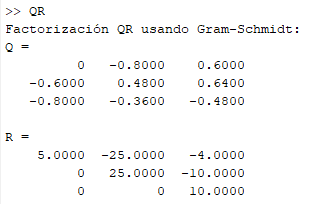
\includegraphics[width=\textwidth]{Figures/qr gs.png}
    \end{minipage}
    \begin{minipage}{0.49\textwidth}
        \centering
        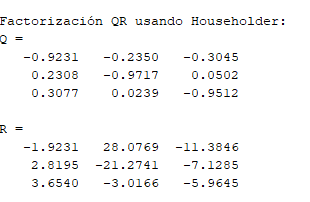
\includegraphics[width=\textwidth]{Figures/qr hh.png}
    \end{minipage}
\end{figure}


Al comparar los métodos de factorización QR mediante Gram-Schmidt y Householder, se observa que el primero produjo una descomposición sin problemas, mientras que el segundo mostró inconsistencias, en particular una matriz \( R \) que no es triangular superior. Esto sugiere que la implementación del método de Householder pudo haber sufrido errores numéricos acumulativos.

Las transformaciones de Householder están diseñadas para introducir ceros en la parte inferior de la matriz mediante reflexiones ortogonales. Sin embargo, pequeños errores en la normalización de los vectores reflejados pueden amplificarse, afectando la estructura triangular de \( R \). Además, la sensibilidad a la escala de los valores de la matriz original puede exacerbar estos errores. En este caso, la segunda columna de la matriz tiene valores significativamente mayores en magnitud que la primera, lo que puede haber llevado a problemas de redondeo y pérdida de precisión en los cálculos.

A pesar de que Householder es generalmente más estable que Gram-Schmidt, la implementación computacional puede verse afectada por la acumulación de errores de redondeo, especialmente si las operaciones no se manejan con la precisión adecuada. Esto explicaría por qué Gram-Schmidt, a pesar de ser teóricamente menos estable, produjo mejores resultados en este caso particular.
\textbf{Nota:} Usando los algoritmos propios de matlab las 2 solciones (QR y Grand-Smith) dan la misma solución teórica.
        \end{solucion}
    \end{itemize}
\end{homeworkProblem}
